\documentclass[tikz,border=10pt]{standalone}

\usepackage{xcolor}
\usetikzlibrary{arrows.meta, positioning, fit}

\definecolor{paperBlue}{RGB}{35,79,140}
\definecolor{paperGreen}{RGB}{34,125,92}
\definecolor{paperGold}{RGB}{176,125,33}
\definecolor{paperSoft}{RGB}{246,248,250}
\definecolor{paperLine}{RGB}{80,92,110}

\begin{document}
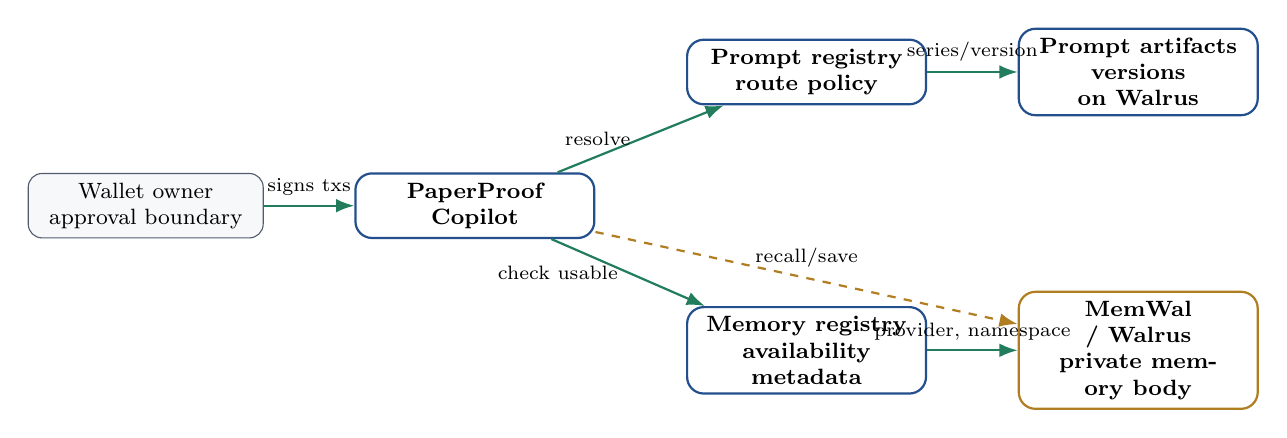
\begin{tikzpicture}[
    node distance=0.85cm and 1.15cm,
    box/.style={draw=paperLine, rounded corners=5pt, fill=paperSoft, minimum height=0.78cm, align=center, font=\footnotesize, text width=2.75cm},
    public/.style={draw=paperBlue, thick, rounded corners=6pt, fill=white, minimum height=0.82cm, align=center, font=\footnotesize\bfseries, text width=2.8cm},
    private/.style={draw=paperGold, thick, rounded corners=6pt, fill=white, minimum height=0.82cm, align=center, font=\footnotesize\bfseries, text width=2.8cm},
    arrow/.style={-Latex, thick, draw=paperGreen},
    dashedarrow/.style={-Latex, thick, dashed, draw=paperGold}
]
    \node[box] (wallet) {Wallet owner\\approval boundary};
    \node[public, right=of wallet] (copilot) {PaperProof\\Copilot};
    \node[public, above right=of copilot] (prompt) {Prompt registry\\route policy};
    \node[public, right=of prompt] (artifact) {Prompt artifacts\\versions on Walrus};
    \node[public, below right=of copilot] (memreg) {Memory registry\\availability metadata};
    \node[private, right=of memreg] (memwal) {MemWal / Walrus\\private memory body};

    \draw[arrow] (wallet) -- node[above, font=\scriptsize] {signs txs} (copilot);
    \draw[arrow] (copilot) -- node[left, font=\scriptsize] {resolve} (prompt);
    \draw[arrow] (prompt) -- node[above, font=\scriptsize] {series/version} (artifact);
    \draw[arrow] (copilot) -- node[left, font=\scriptsize] {check usable} (memreg);
    \draw[dashedarrow] (copilot) -- node[above, font=\scriptsize] {recall/save} (memwal);
    \draw[arrow] (memreg) -- node[above, font=\scriptsize] {provider, namespace} (memwal);
\end{tikzpicture}
\end{document}
